\documentclass[12pt]{beamer}

% Packages
\usepackage{graphicx}
\usepackage{svg}
\usepackage{booktabs}
\usepackage{caption}

\usepackage[style=numeric,citestyle=numeric]{biblatex}
\addbibresource{references.bib}

% Redefine \supercite to use square brackets
\DeclareCiteCommand{\supercite}[\mkbibsuperscript]
  {\iffieldundef{prenote}
     {}
     {\BibliographyWarning{Ignoring prenote argument}}%
   \iffieldundef{postnote}
     {}
     {\BibliographyWarning{Ignoring postnote argument}}}
  {\usebibmacro{citeindex}%
   \bibopenbracket\usebibmacro{cite}\bibclosebracket}
  {\supercitedelim}
  {}


\title{Addressing Data Scarcity in Medical Imaging: Synthetic Data Generation and Self-Supervised Learning}
\author{%
  Scott Chase Waggener, M.S.$^{1,2}$, 
  Timothy Cogan, Ph.D.$^1$, 
  Lakshman Tamil, Ph.D., FNAI$^2$
}

\institute{
  $^1$MedCognetics, Inc., Dallas, TX \and
  $^2$University of Texas at Dallas
}

\date{\today}

\begin{document}

\frame{\titlepage}

\begin{frame}
\frametitle{Problem Statement}
\begin{itemize}
    \item Medical imaging data is relatively scarce compared to other modalities
    \begin{itemize}
        \item EMBED\supercite{embed2023} - 3.4M mammograms
        \item Compare with LAION-5B \supercite{laion5b} - 5.85B image text pairs 
    \end{itemize}
    \item Annotating medical data presents challenges
    \begin{itemize}
        \item Expert labeling is time consuming and costly
        \item Biopsy confirmation, multi-year stability, etc.
        \item Social determinants of health can bias labels
    \end{itemize}
    \item SOTA methods like Vision Transformers \supercite{dosovitskiy2020vit} work best with large amounts of data
\end{itemize}
\end{frame}

\begin{frame}
\frametitle{Synthetic Mammography}
\begin{itemize}
    \item Synthetic data can alleviate data scarcity
    \begin{itemize}
        \item Create aribrarily large volume of data
        \item Vary simulation parameters to represent rare conditions
        \item Establish ground truth from simulation
    \end{itemize}
    \item VICTRE \supercite{victre} is a mammographic simulation pipeline developed by the FDA
    \begin{itemize}
        \item Simulates full-field digital mammography (FFDM)
        \item Produces high-quality synthetic mammograms
    \end{itemize}
\end{itemize}
\end{frame}

\begin{frame}
\frametitle{VICTRE Pipeline}
\begin{enumerate}
    \item \underline{Generate} breast phantom as a voxelized object with known material types
    \item \underline{Insert} simulated lesions into breast phantom (optional)
    \item \underline{Compress} breast phantom to simulate mammographic positioning
    \item \underline{Project} breast phantom into 2D using Monte Carlo ray tracing
    \item \underline{Reconstruct} tomosynthesis slices from 2D projections
    \item \underline{Process} mammogram for final presentation
\end{enumerate}
\vspace{1cm}
\begin{figure}[h!]
\centering
\includesvg[width=1.0\textwidth]{figures/simulator.svg}
\end{figure}
\end{frame}


\begin{frame}
\frametitle{VICTRE Synthetic Mammogram}
\begin{figure}[h!]
\centering
\begin{minipage}{0.48\textwidth}
    \centering
    \includegraphics[width=\textwidth]{figures/projection_DM1.png}
    \captionof*{figure}{Raw VICTRE Projection}
\end{minipage}
\hfill
\begin{minipage}{0.48\textwidth}
    \centering
    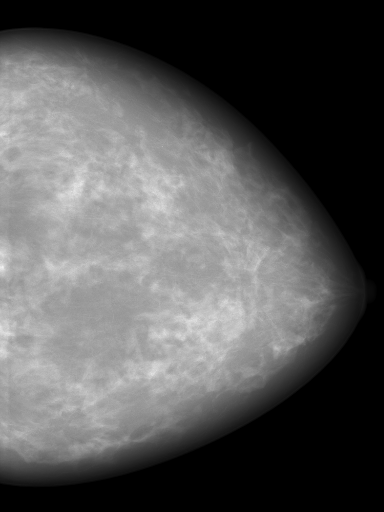
\includegraphics[width=\textwidth]{figures/for_presentation.png}
    \captionof*{figure}{Processed VICTRE Projection}
\end{minipage}
\end{figure}
\end{frame}

\begin{frame}
\frametitle{VICTRE Application}
\begin{itemize}
    \item Estimating percent fibroglandular tissue composition of the breast
    \item Ground truth can be computed from a VICTRE phantom
    \item Trained density algorithm on real mammograms, applied it to synthetic mammograms
    \begin{itemize}
        \item Density categories (A, B, C, D) mapped to density score on interval $I=[0,1]$
        \item Predicted density score compared with VICTRE fibroglandular composition
    \end{itemize}
\end{itemize}
\begin{minipage}[t]{0.5\textwidth}
\begin{figure}[h!]
\centering
\includesvg[width=\textwidth]{figures/synth_density_real.svg}
\end{figure}
\end{minipage}%
\hfill
\begin{minipage}[t]{0.5\textwidth}
\begin{figure}[h!]
\centering
\includesvg[width=\textwidth]{figures/synth_density_synth.svg}
\end{figure}
\end{minipage}
\end{frame}

\begin{frame}
\frametitle{VICTRE Application}
\begin{itemize}
    \item Predicted density score on VICTRE mammograms correlates with percent fibroglandular tissue composition
    \item Indicates that synthetic mammograms can be used to evaluate AI models
\end{itemize}
\begin{figure}[h!]
\centering
\includesvg[width=0.45\textwidth]{figures/synthetic_data_predictions.svg}
\end{figure}
\end{frame}


\begin{frame}
\frametitle{Self-Supervised Learning}
\begin{itemize}
    \item Self-Supervised Learning (SSL) allows models to learn from unlabeled data
    \begin{itemize}
        \item Utilize (large) pool of unlabeled data to pre-train model
        \item Fine-tune on smaller labeled dataset of interest
    \end{itemize}
    \item Popular SSL tasks present issues in the medical imaging domain
    \begin{itemize}
        \item Reliant on augmentations that do not generalize to medical data
        \item Random tissue variations make pixel-level predictions challenging
    \end{itemize}
    \item An ideal medical SSL task should be:
    \begin{itemize}
        \item Generalizable across different imaging modalities
        \item Capable of capturing semantic information
    \end{itemize}
\end{itemize}
\end{frame}

\begin{frame}
\frametitle{Joint-Embedding Predictive Architecture \supercite{lecun2022path}}
\begin{itemize}
    \item Self-supervised learning framework with the properties we desire
    \begin{itemize}
        \item Substantial flexibility in how the task is implemented
        \item No assumptions about input signals
        \item Latent space predictions capture semantic features
    \end{itemize}
    \item Task: predict embeddings of signal y from compatible signal x using a conditioned predictor network
    \item Example implementation:
    \begin{itemize}
        \item Generate embeddings of signal y from teacher network
        \item Mask part of signal y to form signal x
        \item Student network uses signal x to predict embeddings for masked signal y
    \end{itemize}
\end{itemize}
\end{frame}

\begin{frame}
\frametitle{Medical Joint-Embedding Predictive Architecture}
\begin{itemize}
    \item Choose I-JEPA \supercite{assran2023self} as the foundation
    \item Replace MSE loss with cosine similarity loss
    \item Introduce additional cosine distance contrastive loss
\end{itemize}
\vspace{1cm}
\begin{figure}[h!]
\centering
\includesvg[width=0.9\textwidth]{figures/jepa.svg}
\end{figure}
\end{frame}

\begin{frame}
\frametitle{M-JEPA CIFAR-10 Ablations}
\begin{itemize}
    \item M-JEPA pre-training with a linear probe nearly matches accuracy of fully supervised ViT
    \item Following M-JEPA pre-training with supervised fine-tuning yields highest accuracy
\end{itemize}
\begin{table}[H]
    \centering
    \begin{tabular}{lr}
        \toprule
        Method & Accuracy (\%) \\
        \midrule
        Fully Supervised & 80.3 \\
        Linear Probing & 79.29 \\
        \midrule
        Supervised Fine-Tuning & \textbf{87.5} \\
        LoRA \supercite{hu2021lora} Fine-Tuning &  83.7 \\
        M-JEPA Without Stop-Gradient & 85.1 \\
        \bottomrule
    \end{tabular}
    \caption*{Comparison of fine tuning methods on CIFAR-10 \supercite{assran2023self}}
    \label{tab:cifar10-tune-method}
\end{table}
\end{frame}

\begin{frame}
\frametitle{M-JEPA on Mammograms}
\begin{itemize}
    \item M-JEPA pre-training on mammograms in two stages
    \begin{itemize}
        \item Phase 1: ViT backbone, 512x384 
        \item Phase 2: Adaptive ViT backbone, 3072x2304 
        \item Linear probing task: Classify view as mediolateral oblique (MLO) or craniocaudal (CC)
    \end{itemize}
    \item Supervised fine-tuning for breast cancer triage
\end{itemize}
\begin{table}[H]
    \centering
    \small
    \begin{tabular}{l r r}
        \toprule
        Training Stage & Metric & Value \\
        \midrule
        M-JEPA Phase 1 & View Classification Accuracy & \(99.9\dagger\) \\
        M-JEPA Phase 2 & View Classification Accuracy & \(99.49\dagger\) \\
        Supervised Fine-Tuning & Breast Cancer Triage AUROC & \(0.8603\) \\
        \bottomrule
    \end{tabular}
    \normalsize
    \caption*{$^\dagger$Indicates results obtained through linear probing.}
    \label{tab:mammo-val-metrics}
\end{table}
\end{frame}


\begin{frame}
\frametitle{Conclusion}
\begin{itemize}
    \item VICTRE \supercite{victre} provides a high-quality synthetic mammography pipeline
    \begin{itemize}
        \item Synthesize FFDM and tomosynthesis images
        \item Insertion of simulated lesions
        \item Empirical support for use in evaluating AI models
    \end{itemize}
    \item M-JEPA self-supervised framework learns useful features from unlabeled data
    \begin{itemize}
        \item Applicable to arbitrary medical imaging data and beyond
        \item Linear probing accuracy approaching supervised ViT performance
        \item Supervised fine-tuning exceeds purely supervised performance
    \end{itemize}
\end{itemize}
\end{frame}

\begin{frame}
\frametitle{Acknowledgements}
This research was, in part, funded by the National Institutes of Health (NIH) Agreement No. 1OT2OD032581. The views and conclusions contained in this document are those of the authors and should not be interpreted as representing the official policies, either expressed or implied, of the NIH.
\end{frame}

\begin{frame}
\frametitle{References}
\renewcommand*{\bibfont}{\tiny}
\setbeamertemplate{bibliography entry title}{}
\setbeamertemplate{bibliography entry location}{}
\setbeamertemplate{bibliography entry note}{}
\setlength\bibitemsep{0pt}
\printbibliography[heading=none]
\end{frame}

\end{document}
